\section{Discussion}
We have offered a way around the exploration-exploitation dilemma by showing that curiosity is all that is required for animals to explore, in all circumstances. This is a controversial claim. So we will address some of its criticisms as a series of questions.

\subsection*{What about information theory?}
Weaver \cite{Shannon1948} in his classic introduction to the topic, describes information as a communication problem with three levels. 1. The technical problem of transmitting accurately. 2. The semantic problem of meaning. 3. The effectiveness problem of changing behavior. He then describes how Shannon's work addresses only problem A. It has turned out that Shannon's separation of the problem allowed the information theory to have an incredibly broad application. 

Unfortunately valuing information is not at its core a communications problem. Consider for example Bob and Alice having a phone conversation, and then Tom and Bob having the exact same conversation. The personal history of Bob and Alice will determine what Bob learns in their phone call, and so determines if we argue that he values that phone call. These might be completely different from what he learns when talking to Tom, even if the conversations are identical. What we mean by this example is the personal history defines what is valuable on a channel, and this is independent of the channel and the messages sent. We have summarized this diagrammatically, in Fig. ~\ref{fig:info1}.

\begin{figure}
\begin{fullwidth}
	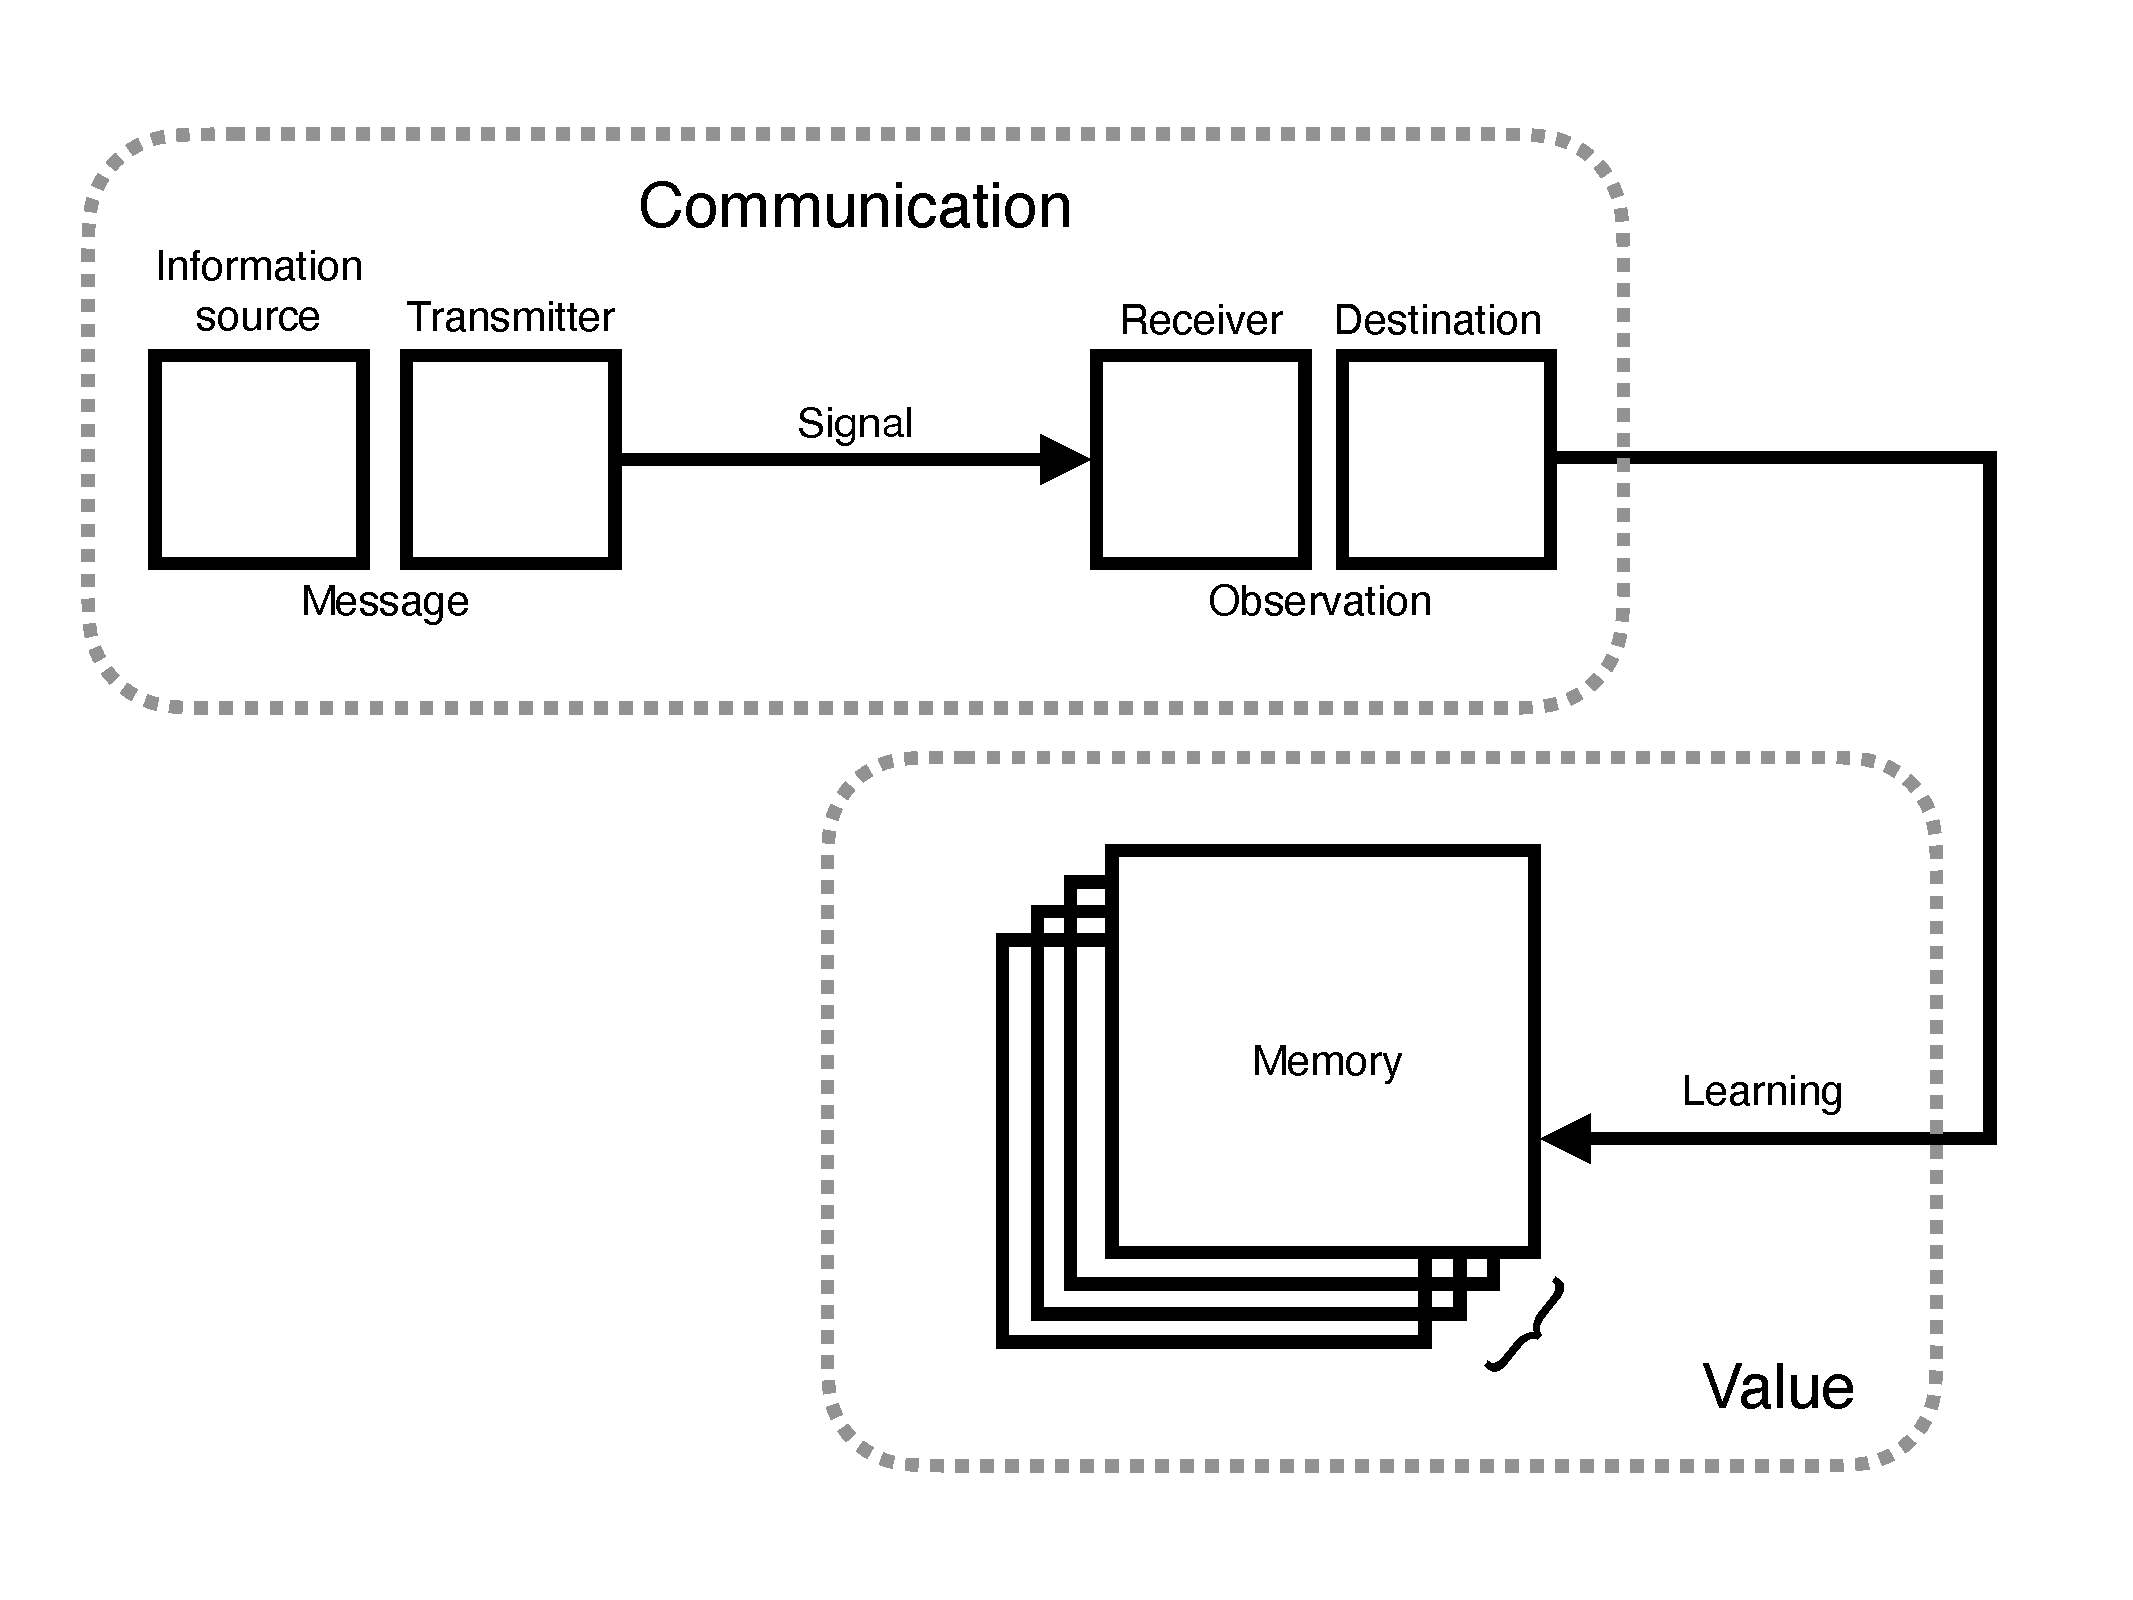
\includegraphics[width=0.7\linewidth]{img/info_diagram.pdf} 
    \caption{The relationship between the technical problem of communication with the technical problem of value. Note how value is not derived from the channel. Value is derived from learning about observations, which is in turn dependent on memory and its past history.
    }
    \label{fig:info1} 
\end{fullwidth}
\end{figure}

There is however an analogous set of levels for information value as to those Weaver describes. a. There is the technical problem of judging how much was learned. b. There is the semantic problem of both what this learning ``means'', and also what its consequences are. c. There is an effectiveness problem of using what was learned to some other effect. In many ways b and c are similar to those in the information theory. It is which is most different. 

For the same reasons Shannon avoided b and c in his theory, we have avoided them. Both of them are very hard to measure which makes them very hard to study mathematically. We feel it necessary to build a theory of information value which can act as a companion for information theory. This is why we took an axiomatic approach, and why we have tried to ape Shannon's axioms, as it made sense to do so.


\subsection*{Is this too complex?}
Perhaps turning a single objective into two, as we have, is an unneeded complication. If this is true this it would mean ours is not a parsimonious solution to the dilemma, and so we could or should reject it on that alone. 

Questions about parsimony are resolved by considering the benefits versus the costs. The benefits to curiosity-based search is that it leads to no regret solutions to exploration, to exploration-exploitation, and that it so far seems to do very well in practice, at reward collection. At the same time curiosity-as-exploration can also be building a model of the environment, useful for later planning \cite{Ahilan2019,Poucet1993}, creativity, imagination \cite{Schmidhuber2010}, while also building, in some cases, diverse action strategies \cite{Lehman2011a,Lehman2013,Mouret2015,Colas2020}. In other words, we argue it is a necessary complexity. 


\subsection*{Is this too simple?}
Solutions to the regular dilemma are complex and require sophisticated mathematical efforts and complex computations when compared to our solution. Or put another way, our solution may seem too simple. So have we ``cheated'' by changing the problem as we have?

The truth is we might be cheating in this sense. The dilemma might have to be as hard as it has seemed in the past. But the general case for curiosity as useful is clear, and backed up by the brute fact of its widespread presence in animals. The question is: is curiosity so useful and so robust that it can be sufficient for all exploration with learning. 

% TODO - add behave cites
% TODO - add ML cites
The answer to this question is empirical. If our account does well in describing and predicting animal behavior, that would be some evidence for it. If it predicts neural structures \cite{Cisek2019}, that would be some evidence for it. If this theory proves useful in machine learning and artificial intelligence research, that would be some evidence for it.


\subsection*{Is this a slight of hand, theoretically?}
Yes. It is often useful in mathematical studies to take one problem that cannot be solved, and replace it with another related problem that can be. This is what we have done for exploration and the dilemma. The regular view of the problem has no tractable solution, without regret. Ours has a solution.


\subsection*{Does value as a technical problem even make sense?}
Information value has been taken up as a problem in meaning, or usefulness \cite{needed}. These are based on what we will call b-type questions (a notion we defined in the section above). It is not that b questions are not important or are not valuable. It is that they are second order questions. The first order questions are the 'technical' or a-type questions (also defined above). 

Having a technical definition for value, free from any meaning, might seem counterintuitive for a value measure. But we argue that it is not more or less counterintuitive than stripping information of meaning in the first  place. (This is how Shannon got his information theory). The central question for our account of value is, is it useful? It is enough to ensure a complete but perfectly efficient search for information/learning in any finite space. It is enough to play a critical part in solving/replacing the dilemma, which has for many years looked intractable. 


\subsection*{What about mutual information, or truth?}
In other prototypical examples, information value is based on how well what is learned relates to the environment \cite{needed}. Their mutual information that is. (Colloquially, one might call this truth.) The larger the mutual information between the environment and the memory, the more value it is said that we should then expect. This view seems to us at odds with actual learning behavior, especially in humans. 

As a people we pursue information which is fictional, or based on analogy, or outright wrong. Conspiracy theories, disinformation, and our many more mundane errors, are far too commonplace for value to be based on fidelity alone. This does not mean that holding false beliefs cannot harm survival. But this is a second order question as far as learning behavior foes. The fact that humans consistently seek to learn false things calls out that learning alone is a motivation. This is what opens the door for a technical definition.


\subsection*{So you suppose there is always positive value for learning of all fictions, disinformationist, and deceptions?}
This is our most unexpected prediction: We must.


\subsection*{What about information foraging?}
Our work is heavily inspired by information foraging. (We are also aware of its limits \cite{needed}). Our motivation in developing was that information value should not depend on only a probabilistic reasoning, as it does in information foraging. This is for the simple reason that many of the problems animals need to learn are not probabilistic problems \textit{from their point of view}. (Most any learning problem can be described as probabilistic from an outsider's perspective; the one scientists' rely on). We also felt the algorithmic curiosity looked so important that it needed as general a way to study it, which is why we developed an axiomatic approach that ended up addressing the technical problem of information value.


\subsection*{Was it necessary to build a general theory for information value just to describe curiosity?}
No. It was an idealistic choice, which worked out. The field of curiosity studies has shown there are many kinds of curiosity. At the extreme limit of this diversity is a notion of curiosity defined for any kind of observation, and any kind of learning. If we were able to develop a theory of value driven search at this limit, we can be sure it will apply in all possible examples of curiosity that we seem sure to discover in future. At this limit we can also be sure the ideas will span fields, addressing the problem as it appears in computer science, psychology, neuroscience, biology, and perhaps economics.


\subsection{Doesn't your definition of regret ignore lost rewards when the curiosity policy is in control?}
Yes. Regret is calculated for the policy which is in control of behavior, not the policy which \textit{could} have been in control of behavior.


\subsection*{Is information a reward?}
It depends. If reward is defined as more-or-less any quantity that motivates behavior, then our definition of information value is a reward. This does not mean however that information value and environmental rewards are interchangeable. In particular, if you add reward value and information value to motivate search you can drive exploration in practical and useful ways. But this doesn't change the intractability of the dilemma proper \cite{Thrun1992a,Dayan1996,Findling2018,Gershman2018b}. So exploration will still generate substantial regret (as we show in Fig \ref{fig:summary}). But perhaps more important is that these kinds of intrinsic rewards \cite{Schmidhuber1991,Berger-Tal2014,Itti2009,Friston2016,Kobayashi2019} introduce a bias that will drive behavior away from what, could otherwise be, ideal skill learning \cite{Ng1999,Simsek2006}.


\subsection*{But isn't curiosity impractical?}
It does seem curiosity is just as likely to lead away from a needed solution, as towards it. Especially so if one watches children who are the prototypical curious explorers \cite{Sumner2019,Kidd2015}. This is why we limit curiosity with boredom, and counter it with a competing drive for reward collecting / exploitation. 

We believe there is a useful analogy between science and engineering. Science can be considered an open-ended inquiry, and engineering a purpose driven enterprise. They each have their own pursuits but they also learn from each other, often in alternating iterations \cite{Gupta2006}. It is their different objectives though which make them such good long-term collaborators.


\subsection*{But what about curiosity on big problems?}
A significant drawback to curiosity, as an algorithm, is that it will struggle to deliver timely results when the problem is very large, or highly detailed. First, it's worth noting that most learning algorithms struggle with this setting \cite{MacKay2003,Sutton2018}, unless that is unless significant prior knowledge can be brought to bear \cite{Zhang2020,Sutton2018} or the problem can be itself compressed \cite{Ha2018a,Fister2019}. Because however ``size'' is a widespread problem in learning, there are a number of possible solutions. And because our definition of learning, memory and curiosity is so general, we can take advantage of most. This does not guarantee curiosity will work out for all problems; all learning algorithms have counterexamples afterall \cite{Wolpert1997}.


\subsection*{But what about other forms of curiosity?}
We did not intend to dismiss the niceties of curiosity, which others have revealed. It is that these prior divisions parcel out the idea too soon. Philosophy and psychology consider whether curiosity is internal or external, perceptual versus epistemic, or specific versus diversive, or kinesthetic \cite{Kidd2015,Berlyne1950,Zhou2020}. Computer science tends to define it as needed, for the task at hand \cite{Stanley2004,Friston2016,Lehman2011a,Lehman2013,Mouret2015,Colas2020}. Before dividing it it is important to first define it, mathematically. 


\subsection*{What is boredom, besides being a tunable parameter?}
A more complete version of the theory would let us derive a useful or even optimal value for boredom, if given a learning problem or environment. This would also answer the question of what boredom is computationally. We cannot do this. It is a next problem we will work on and it is very important. The central challenging comes in deriving boredom while keeping the abstract approach which we have used, and which seems critical.
% TODO - copy old boredom discuss here.


\subsection*{Does this mean you are hypothesizing that boredom is an actively tuned?}
We are predicting exactly that.


\subsection*{But do people subjectively feel they can tune their boredom?}
From our personal experience, we do not. Perhaps it happens unconsciously. The relationship between learning, function, consciousness and unconscious is not well enough understood for how something does or does not feel to be an argument in and of itself.


\subsection*{How can an animal tune boredom in a new setting?}
The short answer is that it would need to guess and check. Our work in Fig \ref{fig:robust} suggests this can be somewhat robust.


\subsection*{Do you have any evidence for this in animal behavior and neural circuits?}
There is some evidence. In psychology and neuroscience, curiosity and reinforcement learning have developed as separate disciplines \cite{Berlyne1950,Kidd2015,Sutton2018}. And er highlighted how they are separate problems, with links to different basic needs: gathering resources to maintain physiological homeostasis \cite{Keramati2014,Juechems2019} and gathering information to decide what to learn and to plan for the future \cite{Valiant1984,Sutton2018}. Here we suggest that though they are separate problems, they are problems that can, in large part, solve one another. This insight is the central idea to our view of the explore-exploit decisions. 

Cisek (2019) has traced the evolution of perception, cognition, and action circuits from the Metazoan to the modern age \cite{Cisek2019}. The circuits for reward exploitation and observation-driven exploration appear to have evolved separately, and act competitively--exactly the model we suggest. In particular he notes that exploration circuits in early animals were closely tied to the primary sense organs (i.e. information) and, historically anyway, had no input from the homeostatic circuits needed for reward valuation \cite{Keramati2014,Cisek2019,Juechems2019}. This neural separation for independent circuits has been observed in ``modern'' high animals, including zebrafish \cite{needed}, mouse \cite{needed}, humans \cite{needed}, and monkey \cite{White2019,Wang2019}. It is difficult to know the exact objectives of these circuits, but their independence aof activity and independence during behavior suggests they are, by degrees, independent policies.


\subsection*{What about aversive values?}
We do not believe this is complete theory. For example, we do not account for any consequences of learning, or any other aversive events. The need to add 
% TODO...


\subsection*{Fitting deterministic models?}
The theoretical description of exploration in scientific settings is probabilistic \cite{Calhoun2014,Song2019a,Gershman2018b,Schulz2018a}. By definition probabilistic models can't make exact predictions of behavior, only statistical ones. Our approach is deterministic, and so does make exact predictions. Our theory predicts that it should be possible to guide exploration in real-time using, for example, optogenetic methods in neuroscience, or well timed stimulus manipulations in economics or other behavioral sciences. 

In species ranging from human to \textit{Caenorhabditis elegans}, there are hundreds perhaps thousands of exploration-exploitation experiments. Analysis of their behavior has generally been limited to distributions. A deterministic theory can, in principle, open up entirely new avenues for reanalysis by using our model to make exact predictions.

\textbf{TODO} - discuss practical fits:
\begin{enumerate}
    \item Burn in
    \item Population E0, and refinement, replicators?
    \item Data fusion (bayes methods for deterministic equations are legit)
\end{enumerate}


\subsection*{Does regret matter?}
Another way around the dilemma is to ignore regret altogether. This is the domain of pure exploration methods, like the Gitten’s Index \cite{needed}, or probably-approximately correct approaches \cite{Valiant1984}, or other bounded forms of reinforcement learning \cite{needed}. Such methods can guarantee that you find the best value, eventually. These methods do not consider regret. But regret is critical for making sure that an animal's actions are efficient when resources and time are scarce, as they are in almost every natural setting. 


\subsection*{Summary}
There will be certainly cases in an animal's life when their exploration must focus on tangible physical rewards. Even here searching for information about physical rewards, rather than searching for their value, will make the search more robust to deception, and more reliable in the future. Think of this as curiosity about reward. There are many more cases where curiosity can include observations of the environment, and the self. This paper has argued that one should put aside intuitions which suggest open-ended curious search is too inefficient to be practical. We have shown how it can be made very practical. This paper has argued one should put aside older intuitions for what exploratory behavior in animals represents. We have showed how there is a zero-regret way to solve the dilemma, a problem which has seemed unsolvable.